\documentclass[12pt,a4paper]{article}
\usepackage[utf8]{inputenc}
\usepackage{amsmath}
\usepackage{amsfonts}
\usepackage{amssymb}

\usepackage{cmap} % для кодировки шрифтов в pdf
\usepackage[T1]{fontenc}
\usepackage{hhline}
\usepackage[unicode]{hyperref}
\usepackage{multirow}
\usepackage{array}
\usepackage{amsmath}
\usepackage{bm}
\usepackage{textcomp}
\usepackage[russian]{babel}
\usepackage{graphicx} % для вставки картинок
\usepackage{amssymb,amsfonts,amsmath,amsthm} % математические дополнения от АМС
\usepackage{indentfirst} % отделять первую строку раздела абзацным отступом тоже
% Поля
\usepackage{geometry}
\geometry{left=2cm}
\geometry{right=1.5cm}
\geometry{top=2.4cm}
\geometry{bottom=2.cm}

%%%%%%%%%%%%%%%%%%%%%%%%%%%%%%%     

\linespread{1.5} % полуторный интервал
\frenchspacing

\begin{document}
	
	\begin{titlepage}
		
		\begin{center}
			\begin{large}
				Санкт-Петербургский Политехнический университет\\ Петра Великого\\
				Институт прикладной математики и механики\\
			\end{large}
			\vspace{0.2cm}
			Высшая школа прикладной математики и вычислительной физики\\
			
		\end{center}
		
		\vspace{3cm}
		\begin{center}
			\textbf{Отчёт\\ по лабораторной работе 3\\ по дисциплине\\ "математическая статистика"}
		\end{center}
		
		\vspace{3cm}
		\vbox{%
			\hfill%
			\vbox{%0
				\hbox{Выполнил студент:}%
				\hbox{\break}
				\hbox{Аникин Александр Алексеевич,}%
				\hbox{группа 3630102$\backslash$80201}%
				\hbox{\break}
				\hbox{\break}
				\hbox{Проверил:}
				\hbox{\break}
				\hbox{к.ф.-м.н., доцент}
				\hbox{Баженов Александр Николаевич}
			}%
		} 
		\vfill
		
		\begin{center}
			Санкт-Петербург\\2021
		\end{center}
		
	\end{titlepage}
	\tableofcontents
	\newpage
	
	\listoffigures
	\newpage
	
	\listoftables
	\newpage	
	
	\section{Постановка задачи}
	Для следующих распределений:
	\begin{itemize}
		\item Нормальное распределение $\textit{N}(\textit{x}, 0, 1)$
		\item Распределение Коши $\textit{C}(\textit{x}, 0, 1)$
		\item Распределение Лапласа $\textit{L}(\textit{x}, 0, \frac{1}{\sqrt{2}})$
		\item Распределение Пуассона $\textit{P}(\textit{k}, 10)$
		\item Равномерное распределение $\textit{U}(\textit{x}, -\sqrt{3}, \sqrt{3})$
	\end{itemize}
	Сгенерировать выборки размером 20 и 100 элементов.
	Построить для них боксплот Тьюки.
	Для каждого распределения определить долю выбросов экспериментально (сгенерировав выборку, соответствующую распределению 1000
	раз, и вычислив среднюю долю выбросов) и сравнить с результатами,
	полученными теоретически.
	
	\newpage
	
	\section{Теория}
		\subsection{Рассматриваемые распределения}
			Плотности:
			\begin{itemize}
				\item Нормальное распределение:
				\begin{equation}\label{norm}
					\textit{N}(\textit{x}, 0, 1)=\frac{1}{\sqrt{2\pi}}e^{-\frac{x^2}{2}}
				\end{equation}
				
				\item Распределение Коши:
				\begin{equation}\label{cauchy}
					\textit{C}(\textit{x}, 0, 1)=\frac{1}{\pi}\frac{1}{x^2+1}
				\end{equation}
				
				\item Распределение Лапласа:
				\begin{equation}\label{laplace}
					\textit{L}(\textit{x}, 0, \frac{1}{\sqrt{2}})=\frac{1}{\sqrt{2}}e^{-\sqrt{2}|x|}
				\end{equation}
				
				\item Распределение Пуассона:
				\begin{equation}\label{poisson}
					\textit{P}(\textit{k}, 10)=\frac{10^k}{k!}e^{-10}
				\end{equation}
				
				\item Равномерное распределение:
				\begin{equation}\label{uniform}
					\textit{U}(\textit{x}, -\sqrt{3}, \sqrt{3})=
					\left\{
					\begin{array}{l}
						\frac{1}{2\sqrt{3}} \quad \text{при} \quad |x|\leq \sqrt{3}\\
						0 \quad \quad \text{при} \quad |x|>3
					\end{array}
					\right.
				\end{equation}
			\end{itemize}
		
		\subsection{Боксплот Тьюки}
			\subsubsection{Построение}
				Границами ящика – первый и третий квартили, линия в середине ящика —
				медиана. Концы усов — края статистически значимой выборки (без выбросов). Длина «усов»:
				\begin{equation}\label{boxplot}
					X_1=Q_1 - \frac{3}{2}(Q_3-Q_1), \quad X_2=Q_3+\frac{3}{2}(Q_3-Q_1),
				\end{equation}
	
				где $X_1$ - нижняя граница, $X_2$ - верхняя граница, $Q_1$ - первый квартиль, $Q_2$ - нижний квартиль.\\
				Данные, выходящие за границы усов (выбросы), отображаются на графике
				в виде маленьких кружков \cite{boxplot_ref}.
				
		\subsection{Теоретическая доля выбросов}
			Можно вычислить теоретические первый и третий квартили распределений - $Q^{T}_{1} и Q^{T}_{2}$. По формуле (\ref{boxplot}) можно вычислить теоретические нижнюю и верхнюю границы уса - $X^{T}_{1} и X^{T}_{2}$. Под выбросами понимаются такие величины $x$, что
			\begin{equation}
				\left[
					\begin{array}{l}
						x < X^{T}_{1} \\
						x > X^{T}_{2}
					\end{array}
				\right.
			\end{equation}
	
			Теоретическая вероятность выбросов:
			\begin{itemize}
				\item для непрерывных распределений:
				\begin{equation}
					P^{T}_{B} = P(x<X^{T}_{1}) + P(x>X^{T}_{2})=F(X^{T}_{1}) + (1-F(X^{T}_{2}))
				\end{equation}
			
				\item для дискретных распределений:
				\begin{equation}
					P^{T}_{B} = P(x<X^{T}_{1}) + P(x>X^{T}_{2})=(F(X^{T}_{1})-P(x=X^{T}_{1})) + (1-F(X^{T}_{2}))
				\end{equation}
			\end{itemize}
			В формулах выше $F(X) = P(x \leq X)$ - функция распределения.

			Теоретические доли выбросов для данных распределений - постоянные величины. Их значения приведены в следующей таблице.
			\begin{table}[h]
				\label{theoretical_outburst}
				\begin{center}
					\begin{tabular}{|c|c|}
						\hline
						Нормальное распределение & 0.007 \\ \hline
						Распределение Коши & 0.156 \\ \hline
						Распределение Лапласа & 0.063 \\ \hline
						Распределение Пуассона & 0.008 \\ \hline
						Равномерное распределение & 0 \\ \hline
					\end{tabular}
				\end{center}
			\caption{Теоретические доли выбросов}
			\end{table}
			
	\newpage
	
	\section{Реализация}
	Лабораторная работа выполнена на языке Python 3.8 с помощью загружаемых пакетов SciPy, MatPlotLib, Pandas, Seaborn. Исходный код лабораторной работы находится на GitHub репозитории.
	\newpage
	
	\section{Результаты}
		\subsection{Боксплоты}
			\begin{figure}[htp]
				{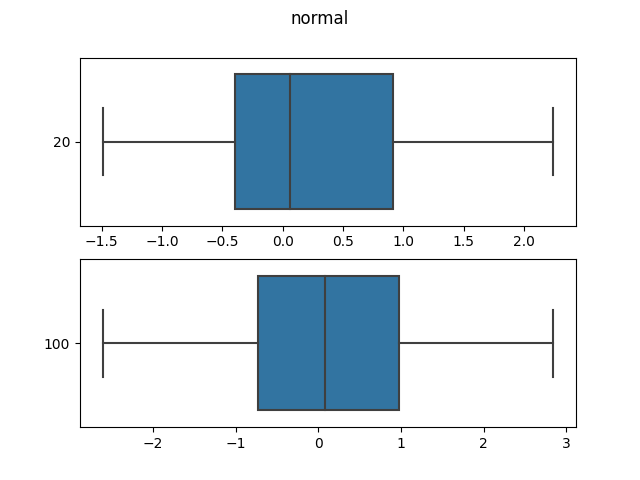
\includegraphics[width=1\linewidth]{../plots/normal.png}}
				\caption{Боксплоты для нормального распределения (\ref{norm})}
			\end{figure}
			\newpage
		
			\begin{figure}[htp]
				{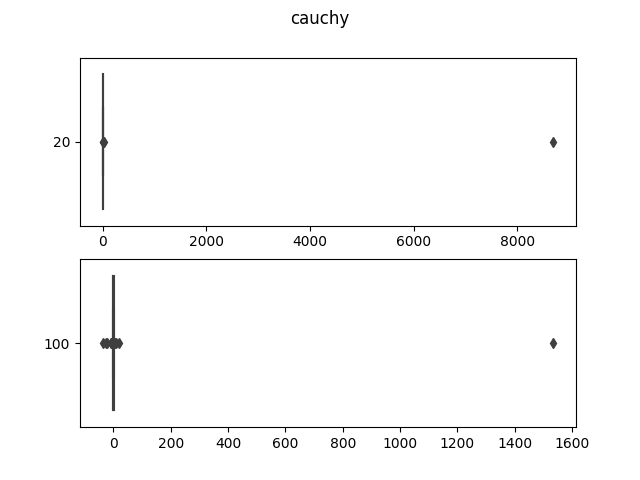
\includegraphics[width=1\linewidth]{../plots/cauchy.png}}
				\caption{Боксплоты для распределения Коши (\ref{cauchy})}
			\end{figure}
			\newpage
			
			\begin{figure}[htp]
				{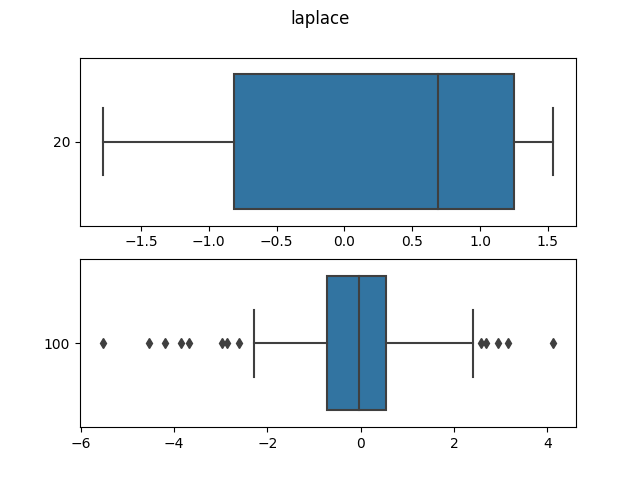
\includegraphics[width=1\linewidth]{../plots/laplace.png}}
				\caption{Боксплоты для распределения Лапласа (\ref{laplace})}	
			\end{figure}
			\newpage
		
			\begin{figure}[htp]
				{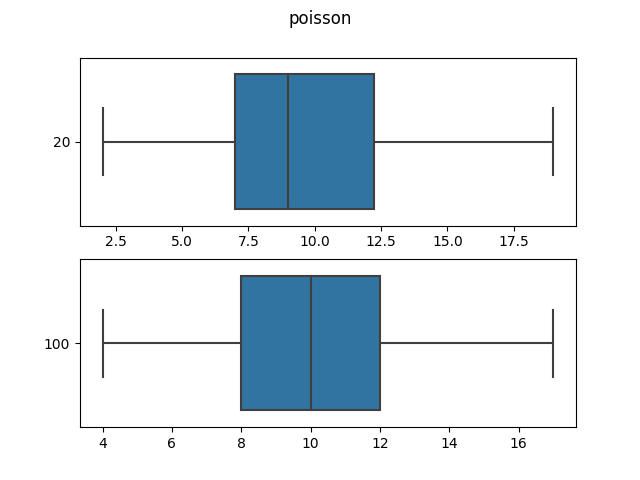
\includegraphics[width=1\linewidth]{../plots/poisson.png}}
				\caption{Боксплоты для распределения Пуассона (\ref{poisson})}
			\end{figure}
			\newpage
			
			\begin{figure}[htp]
				{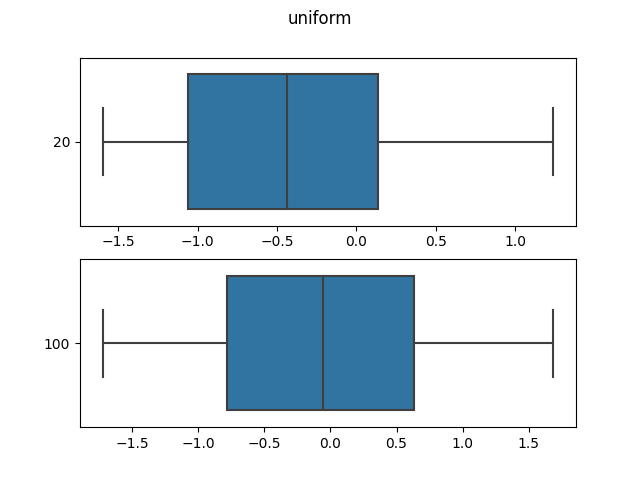
\includegraphics[width=1\linewidth]{../plots/uniform.png}}
				\caption{Боксплоты для равномерного распределения (\ref{uniform})}
			\end{figure}
			\newpage

		\subsection{Эмпирическая и теоретическая доли выбросов}
			\begin{table}[h]
				\label{th_and_emp_outburst}
				\begin{center}
					\begin{tabular}{|c|c|c|c|}
						\hline
						Распределение & Эмп. ДВ, $n=20$ & Эмп. ДВ, $n=100$ & Теор. ДВ \\ \hline
						Нормальное & 0.0248 & 0.0101 & 0.007 \\ \hline
						Коши & 0.1509 & 0.1564 & 0.156 \\ \hline
						Лапласа & 0.0725 & 0.0646 & 0.063 \\ \hline
						Пуассона & 0.0646 & 0.0110 & 0.008 \\ \hline
						Равномерное & 0.0018 & 0.0 & 0 \\ \hline
					\end{tabular}
				\end{center}
				\caption{Эмпирические и теоретические доли выбросов}
			\end{table}
			Нетрудно заметить, что при увеличении размера выборки эмпирическая доля выбросов стремится к теоретической.

	\newpage

	\begin{thebibliography}{1}
		\addcontentsline{toc}{section}{\bibname}
		\bibitem{boxplot_ref}  Box plot. URL: \url{https://en.wikipedia.org/wiki/Box_plot}
	\end{thebibliography}
\end{document}